\documentclass{math}

\usepackage{graphicx}
\usepackage{listings}

\title{Principles of Data Mining: HW 01}
\author{Alvin Lin}
\date{August 2018 - December 2018}
\begin{document}

\maketitle

\subsubsection*{Question 1a}
Filtering out the durations less that half a second removes noise from the data.
Stops that occur for less than half a second are negligible given the scale of
data we are analyzing. These data points represent measurement error in the GPS
tracking and can be filtered out because they are meaningless to our analysis.

\subsubsection*{Question 1d}
Cluster information:
\begin{lstlisting}
Cluster 0
Num points: 120
Average value: 16.346666666666668
Standard deviation: 14.852171184338296
Min: 2.6
Max: 55.2
--------------------
Cluster 1
Num points: 60
Average value: 94.72000000000003
Standard deviation: 25.755658278004336
Min: 56.7
Max: 159.7
--------------------
Cluster 2
Num points: 90
Average value: 1052.5222222222224
Standard deviation: 111.96726582927687
Min: 902.1
Max: 1339.4
--------------------
Cluster 3
Num points: 90
Average value: 3296.5366666666664
Standard deviation: 681.614621395404
Min: 2406.7
Max: 5435.8
--------------------
Thresholds
1339.4
159.7
55.2
\end{lstlisting}
The thresholds calculated by Otsu's method correspond with the max value in the
first three clusters because that is the separation point between the four
clusters we found. This makes sense and creates a visualization that more or
less splits the data into distinct clusters.

\subsubsection*{Question 2}
\begin{center}
  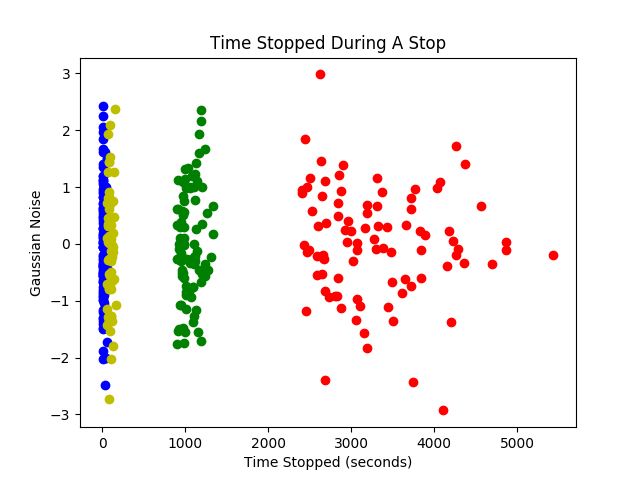
\includegraphics[width=15cm]{assets/hw_01_analysis.png}
\end{center}
This plot shows the time stopped at a given stop plotted against random noise.
Each of the four clusters separated by Otsu's Method is colored with a different
color. The blue and yellow groups most likely represent stops for stop lights
and stop signs since they are short durations averaging 16 and 94 seconds,
respectively. The green group likely represents the cluster of times where the
car was stopped for short term parking (errands), while the red group likely
represents long term parking. \par

\subsubsection*{Question 3}
The blue, yellow, and green clusters are much closer together and have much
smaller standard deviations compared to the red cluster. Long term parking
varies anywhere from 2406 seconds to 5435 seconds, so there are likely a larger
variety of reasons for long term parking. \par
Stopping for a stop light versus stopping for a stop sign are virtually
indistinguishable from each other as their clusters are adjacent to each other.
If we were given a new data point near the existing blue and yellow clusters to
classify as stopping at a stop sign or stopping at a stop light, we would
probably not have a very high accuracy rate.

\begin{center}
  If you have any questions, comments, or concerns, please contact me at
  alvin@omgimanerd.tech
\end{center}

\end{document}
